\section{Fundamentos}

\begin{frame}[fragile]{Definição de árvore}

    \begin{itemize}
        \item Uma árvore é um grafo não direcionado, conectado e acíclico com $N$ vértices e 
        $N - 1$ arestas

        \item A remoção de qualquer uma das arestas divide a árvore em dois componentes

        \item A adição de uma aresta cria um ciclo, descaracterizando a árvore

        \item Para quaisquer vértices $u$ e $v$ da árvore existe um caminho único de $u$ a $v$
    \end{itemize}

\end{frame}

\begin{frame}[fragile]{Visualização de uma árvore}

    \begin{tikzpicture}

        \begin{scope}{shift={(3,0)}}
            \node[opacity=0] (X) at (-1.5, 0) { $1$ };
            \node[circle,draw] (A) at (0, 0) { $1$ };
            \node[circle,draw] (B) at (0, 4) { $3$ };
            \node[circle,draw] (C) at (2, 2) { $7$ };
            \node[circle,draw] (D) at (4, 3) { $4$ };
            \node[circle,draw] (E) at (4, 1) { $2$ };
            \node[circle,draw] (F) at (6, 5) { $5$ };
            \node[circle,draw] (G) at (7, 2) { $6$ };

            \draw (A) -- (C);
            \draw (B) -- (C);
            \draw (C) -- (D);
            \draw (D) -- (E);
            \draw (D) -- (F);
            \draw (F) -- (G);

        \end{scope}
    \end{tikzpicture}

\end{frame}

\begin{frame}[fragile]{Folhas e raiz}

    \begin{itemize}
        \item Uma folha é um nó com apenas um vizinho (no exemplo anterior, os nós com rótulos 
            1, 2, 3 e 6 são folhas da árvore)

        \item Em uma árvore com raiz, um dos nós é escolhido para ser a raiz da árvore

        \item Os demais nós são organizados em níveis, de acordo com sua distância até à raiz

        \item Esta organização é implícita: não é preciso alterar a estrutura da árvore (no
            máximo, deixar indicada qual é a raiz)

        \item Em uma árvore com raiz, os filhos são os vizinhos que estão no nível inferior em
            relação ao nó

        \item Cada nó tem um único pai, o qual é o nó que está no nível imediatamente acima

        \item A estrutura de uma árvore é recursiva: cada nó pode ser interpretado como
            raiz de uma subárvore
    \end{itemize}

\end{frame}

\begin{frame}[fragile]{Visualização de uma árvore com raiz}

    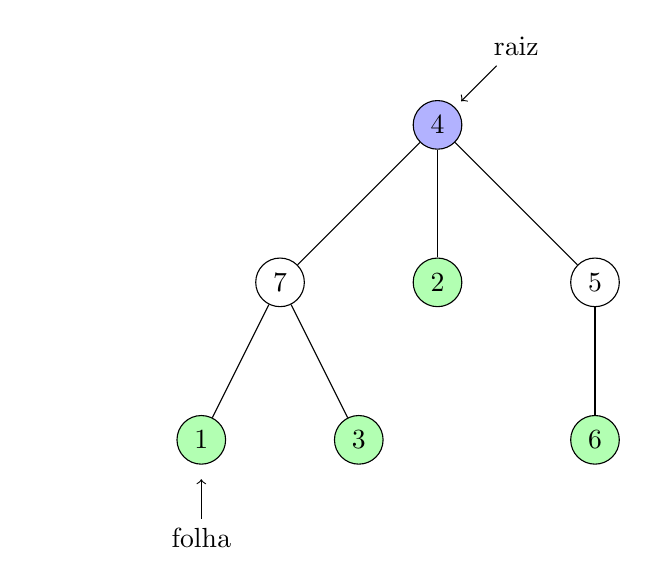
\begin{tikzpicture}

        \begin{scope}{shift={(3,0)}}
            \node[opacity=0] (X) at (-1, 0) { $1$ };

            \node[fill=blue!30,circle,draw] (D) at (4, 5) { $4$ };
            \node[circle,draw] (C) at (2, 3) { $7$ };
            \node[circle,draw,fill=green!30] (E) at (4, 3) { $2$ };
            \node[circle,draw] (F) at (6, 3) { $5$ };
            \node[circle,draw,fill=green!30] (A) at (1, 1) { $1$ };
            \node[circle,draw,fill=green!30] (B) at (3, 1) { $3$ };
            \node[circle,draw,fill=green!30] (G) at (6, 1) { $6$ };

            \draw (A) -- (C);
            \draw (B) -- (C);
            \draw (C) -- (D);
            \draw (D) -- (E);
            \draw (D) -- (F);
            \draw (F) -- (G);

            \node at (5, 6) { raiz };
            \draw[->] (4.75, 5.75) -- (4.3, 5.3);

            \node at (1, -0.25) { folha };
            \draw[->] (1, 0) -- (1, 0.5);

        \end{scope}
    \end{tikzpicture}

\end{frame}


